\chapter{Hardware}
\label{ch:funplenop}
W tym rozdziale zostanie omówiona część projektu związana z oprogramowaniem

\lipsum[1]

\begin{figure}[h!]
  \centering
    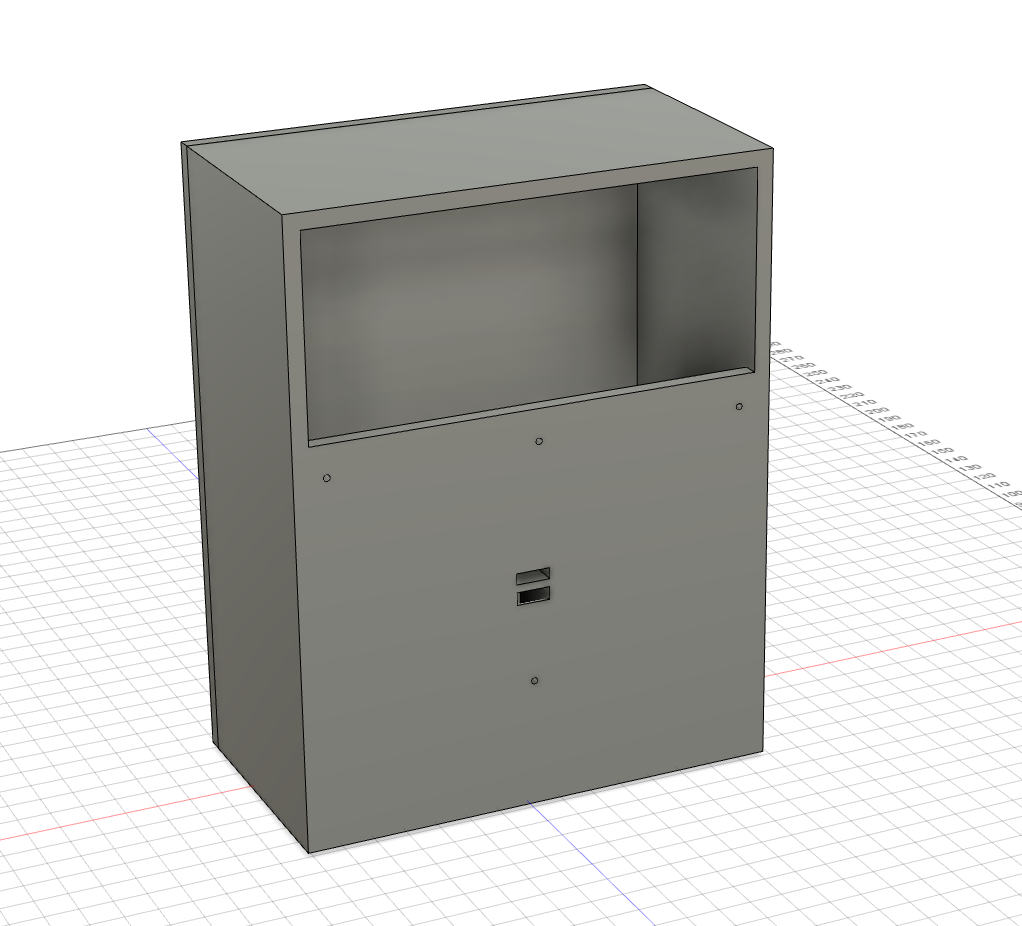
\includegraphics[width=0.5\textwidth]{images/3D/gate_front.png}
  \caption{Zarządzanie zasobami w panelu administratora}
  \label{fig:mobile}
\end{figure}

\begin{figure}[h!]
  \centering
    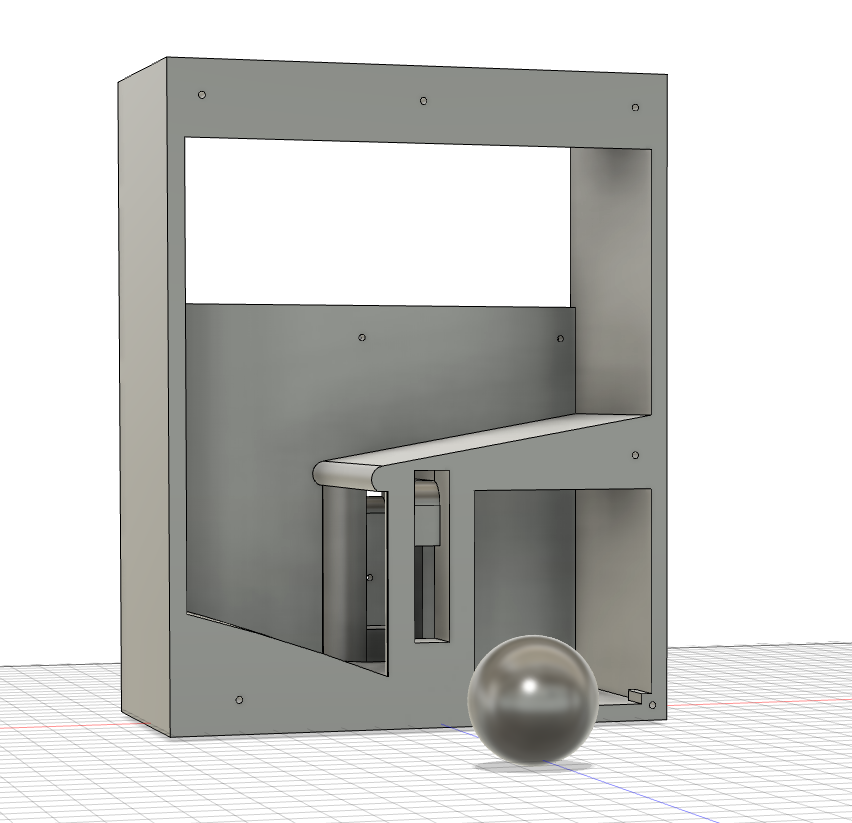
\includegraphics[width=0.5\textwidth]{images/3D/gate_inside.png}
  \caption{Zarządzanie zasobami w panelu administratora}
  \label{fig:mobile}
\end{figure}

\begin{figure}[h!]
  \centering
    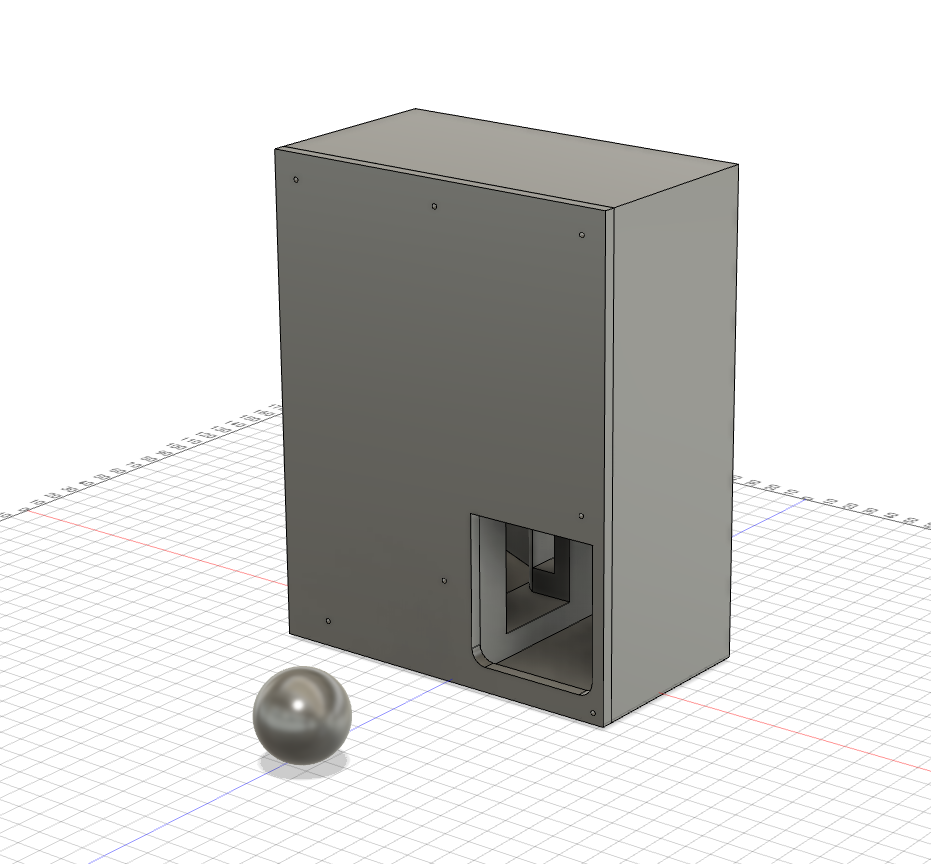
\includegraphics[width=0.5\textwidth]{images/3D/gate_with_back.png}
  \caption{Zarządzanie zasobami w panelu administratora}
  \label{fig:mobile}
\end{figure}

\section{Projekt modelu}
- jaki celu projektu
- w czym projektowane
- co uwzględnia projekt

\section{Druk 3D}
- ?

\section{Raspberry}

\subsection{Czym jest i dlaczego?}

\subsection{Czujniki}
